\chapter{Introducción específica} % Main chapter title

\label{Chapter2}

%----------------------------------------------------------------------------------------
%	SECTION 1
%----------------------------------------------------------------------------------------
En este capítulo se detallan los requerimientos asociados al desarrollo y la implementación de los modelos, así como el contexto y las necesidades de negocio. Finalmente se especificarán las tecnologías aplicadas en el desarrollo del trabajo,
destacando los componentes de inteligencia artificial seleccionados para la predicción de la mora y la rotación. 

\section{Requerimientos asociados al desarrollo e implementación de/los modelo/s}
\label{sec:ejemplo}

\subsection{Requerimientos asociados al desarrollo}

\begin{enumerate}

\item Los códigos deben desarrollarse con herramientas de Microsoft Azure que es el servicio de computación en la nube utilizado por el área de data \textit{analytics}.
\item El equipo de desarrollo tiene la potestad de utilizar el lenguaje de su conocimiento para el desarrollo del código del modelo.
\item Se utiliza GIT como repositorio para el control de versionado de código.


\end{enumerate}


\subsection{Requerimientos asociados a la implementación}
\label{subsec:ejemplo}

\begin{enumerate}
\item Se utiliza Azure Databricks como herramienta tanto para el entrenamiento de los modelos como para su implementación.
\item Debe existir un archivo de ejecución principal llamado \textit{main.py} y un \textit{job} de ejecución automática de ese archivo en Databricks para la implementación \textit{batch}, es decir sin supervisión.
\item Utilización de MLflow, una plataforma de código abierto para la administración del ciclo de vida de los modelos de aprendizaje automático, para el despliegue en producción y el seguimiento de los desarrollos dentro de la compañía.
\end{enumerate}


\section{Modelos de inteligencia artificial utilizados}\label{sec:Modelos}

Como se desarrollará en los próximos capitulos, el modelo elegido para el planteo de la solución fue la regresión logística.
La regresión logística es un modelo de clasificación, también conocida como regresión logit o clasificador de máxima entropía y se encuadra dentro de los modelos lineales generalizados.
La regresión logística describe la probabilidad de que la variable objetivo pertenezca a una clase o a otra: dado un cierto valor límite, si el valor de la variable objetivo iguala o excede dicho valor, se devuelve como predicción la clase "positiva", caso contrario se devuelve como predicción la clase "negativa". Para ello se utiliza la función logística o también llamada función sigmoide, que siempre devuelve un valor entre 0 y 1. A continuación se detalla la función:

\begin{center}
\begin{LARGE}
función sigmoide = $f(x)$ = $\frac{1}{1+e^{-x}}$

\end{LARGE}
\end{center}

En la figura \ref{fig:funcionlog} se puede observar la curva logística:

\vspace{1cm}
\begin{figure}[htbp]
	\centering
	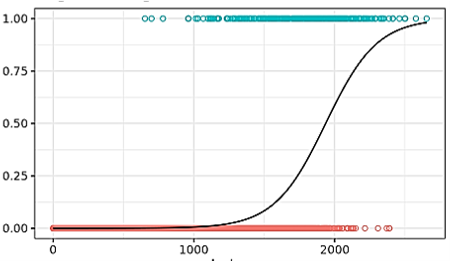
\includegraphics[width=0.8\textwidth]{./Figures/funcionlog.png}
	\caption{Gráfico función logística}
	\label{fig:funcionlog}
\end{figure}
\vspace{1cm}

\vspace{1cm}

La variable ''Y'' a predecir es cualitativa debido a que el objetivo es predecir la probabilidad que un sujeto tome una determinada decisión de índole discreta, condicionada a ciertas variables explicativas y permitiendo identificar las características del sujeto con variables independientes cualitativas.


Para valores de x muy grandes positivos, el valor de $e^{-x}$ es aproximadamente 0 por lo que el valor de la función sigmoide es 1. Para valores de x muy grandes negativos, el valor de $e^{-x}$ tiende a infinito por lo que el valor de la función sigmoide es 0. 

Un punto importante a tener en cuenta a la hora de implementar este modelo es que el set de datos con los que se trabaje debe ser normalizado porque de lo contrario podrían encontrarse indeterminaciones matemáticas.

\section{Herramientas de software utilizadas}
\subsection{Espacio de trabajo: Databricks}
Databricks es una plataforma que facilita la creación y ejecución de \textit{pipelines} o canales de datos permitiendo la colaboración en proyectos de ciencia de datos y analíticos para la construcción e implementación de modelos de aprendizaje de máquina.
Al mismo tiempo, ofrece soluciones de ingeniería de datos, administración, seguridad, gobernanza, entre otros. Está basado en código y estándares abiertos para maximizar su flexibilidad. El enfoque unificado simplifica la arquitectura de datos al eliminar los silos de datos que tradicionalmente separan la analítica, la inteligencia de negocios, la ciencia de datos y el aprendizaje automático.
En la figura  \ref{fig:databricks} se puede visualizar la arquitectura de Databricks:

\vspace{1cm}
\begin{figure}[htbp]
	\centering
	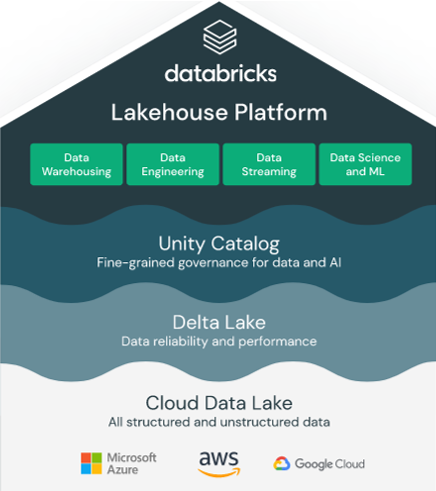
\includegraphics[width=0.7\textwidth]{./Figures/databricks.png}
	\caption{Arquitectura general de la plataforma Databricks.}
	\label{fig:databricks}
\end{figure}
\vspace{1cm}


En cuanto a la terminología utilizada dentro de la plataforma, se pueden detallar los siguientes conceptos clave:

\begin{itemize}
\item Espacio de trabajo: permiten organizar todo el trabajo realizado dentro de la plataforma similar a una estructura de carpetas que permite guardar archivos, bibliotecas utilizadas para la operación y manipulación de datos e incluso compartirlas con otros usuarios.
\item \textit{Notebooks}: se podría definir como conjunto de celdas que permiten ejecutar determinados comandos. Soporta cualquier tipo de lenguaje de programación como Scala, Python, R, SQL, entre otros. Los \textit{notebook} deben estar conectados a un cluster para ejecutar comandos. Se pueden compartir o descargar de forma local.
\item Librerías: son paquetes o módulos que proporcionan una funcionalidad adicional para la resolución de problemas de negocio. Facilitan la programación al proporcionar funcionalidades comunes, que han sido resueltas previamente por otros programadores.
\item Tablas: son datos estructurados utilizados para el análisis, representados por una colección de filas y columnas almacenados como archivos de datos en el almacenamiento de objetos o base de datos.
\item \textit{Clusters}: son grupos de ordenadores que se tratan como un único ordenador. Permiten ejecutar \textit{notebooks} o bibliotecas sobre un conjunto de datos. Cada clúster tiene controles de acceso para garantizar la seguridad de la información 
\item \textit{Jobs}: Los \textit{jobs} son la herramienta mediante la cual se puede programar la ejecución para que se produzca en un clúster ya existente o en un clúster propio. 
\item Aplicaciones: son integraciones de terceros con la plataforma Databricks.Entre ellas se encuentran aplicaciones como Power BI
\end{itemize}
 
\subsection{Motor de análisis y procesamiento: Spark}
Es un motor de análisis unificado para el procesamiento de datos a gran escala. Proporciona una interfaz de programación de aplicaciones de alto nivel, conocida también por la sigla API que es un conjunto de subrutinas, funciones y procedimientos que ofrece la biblioteca para ser utilizada por otro software como capa de abstracción. 
Es compatible con Spark SQL para consultas y procesamiento de datos en SQL, MLlib para el aprendizaje automático o GraphX para procesamiento de gráficos.
Como se menciona en la sección \ref{sec:Modelos}, para el presente trabajo se utilizó la regresión logística como método para predecir la mora y la rotación de un cliente. A continuación se muestra mediante un ejemplo, cómo cargar un conjunto de datos de muestra, construir un modelo de regresión logística y hacer predicciones con el modelo resultante para calcular el error de entrenamiento:

\begin{lstlisting}
from pyspark.mllib.classification import LogisticRegressionWithLBFGS, LogisticRegressionModel
from pyspark.mllib.regression import LabeledPoint

# Load and parse the data 
def parsePoint(line):
    values = [float(x) for x in line.split(' ')]
    return LabeledPoint(values[0], values[1:])

data = sc.textFile("data/mllib/sample_svm_data.txt")
parsedData = data.map(parsePoint)

# Build the model
model = LogisticRegressionWithLBFGS.train(parsedData)

# Evaluating the model on training data
labelsAndPreds = parsedData.map(lambda p: (p.label, model.predict(p.features)))
trainErr = labelsAndPreds.filter(lambda lp: lp[0] != lp[1]).count() / float(parsedData.count())
print("Training Error = " + str(trainErr))

# Save and load model
model.save(sc, "target/tmp/pythonLogisticRegression")
sameModel = LogisticRegressionModel.load(sc,
                                         "target/tmp pythonLogisticRegression")
\end{lstlisting}

\subsection{Lenguaje de programación: Python}
\textit{Python} es un lenguaje de programación que permite trabajar rápidamente e integrar sistemas de forma más eficaz. Entre sus ventajas de uso se puede enumerar:
\begin{enumerate}
\item Amigable y fácil de aprender: existe una comunidad que organiza conferencias y reuniones para facilitar la colaboración entre los programadores. Cuenta con una extensa y detallada documentación que incluye especificaciones de versiones, tutoriales, librerías, módulos, reporte de errores, entre otros.
\item Variedad de aplicaciones: el índice de paquetes de \textit{Python} (PyPI) alberga miles de módulos de terceros para \textit{Python}. Tanto la biblioteca estándar de \textit{Python} como los módulos aportados por la comunidad permiten un sinfín de posibilidades.
\item Código abierto: \textit{Python} está desarrollado bajo una licencia de código abierto aprobada por la OSI (\textit{Open Source Initiative}), lo que hace que se pueda utilizar y distribuir libremente, incluso para uso comercial. La licencia de \textit{Python} es administrada por la \textit{Python Software Foundation}.
\end{enumerate}


\subsection{Gestión del código y versiones: GitHub}
GitHub es una plataforma de alojamiento de código para el control de versiones y la colaboración.Permite trabajar de forma colaborativa en proyectos desde cualquier lugar. A continuación, se enumeran los conceptos escenciales referidos a la plataforma:

\begin{itemize}
\item Repositorios: un repositorio contiene todos los archivos de un proyecto y el historial de revisiones de cada archivo. Existe la posibilidad de discutir y gestionar el trabajo del proyecto dentro del repositorio.
\item Ramas: una rama es una versión paralela de un repositorio. Está contenida dentro del repositorio, pero no afecta a la rama primaria o principal, lo que le permite trabajar libremente sin interrumpir la versión "viva". Cuando se hayan realizado cambios, se puede  fusionar dicha rama de nuevo con la rama principal para publicar los cambios o dicho de otra manera, realizar un \textit{pull request}.
\item \textit{Commits}: un commit, o "revisión", es un cambio individual en un archivo (o conjunto de archivos). Cuando se hace un commit para guardar el trabajo realizado, Git crea un ID único (también conocido como "SHA" o "\textit{hash}") que permite mantener un registro de los cambios específicos confirmados junto con quién los hizo y cuándo. Los \textit{commits} suelen contener un mensaje de \textit{commit} que es una breve descripción de los cambios realizados.
\item Pull requests: las solicitudes de incorporación de cambios permiten comunicar acerca de los cambios insertados en una rama de un repositorio en GitHub. Una vez que se abre una solicitud de incorporación de cambios, se puede debatir y revisar los posibles cambios con los colaboradores y agregar confirmaciones de seguimiento antes de que los cambios se fusionen en la rama base.
\end{itemize}

\subsection{Creación del proyecto, seguimiento y registro del modelo: MLFlow}
MLFlow es una plataforma de código abierto para el ciclo de vida del aprendizaje automático incluyendo la experimentación, la reproducibilidad, el despliegue y un registro central de modelos. Trabaja perfectamente integrado con Python, Apache Spark, Azure Machine Learning, Databricks, entre otros.
Aborda cuatro funciones principales:
\begin{enumerate}
\item MLflow Tracking: seguimiento de experimentos para registrar y comparar parámetros y resultados.
\item MLflow Projects: empaquetado del código de forma reutilizable y reproducible para compartirlo con otros científicos de datos o transferirlo a producción. 
\item MLflow Models: gestión y despliegue de modelos desde una variedad de bibliotecas de aprendizaje automático a una variedad de plataformas de inferencia y servicio de modelos. 
\item MLflow Model Registry: proporciona un almacén central de modelos para gestionar de forma colaborativa el ciclo de vida completo de un modelo MLflow, incluyendo el versionado de modelos, las transiciones de etapas y las anotaciones.
MLflow es agnóstico a las librerías. Se puede utilizar con cualquier biblioteca de aprendizaje automático, y en cualquier lenguaje de programación, ya que todas las funciones son accesibles a través de una API REST y CLI.
\end{enumerate}

\subsection{Programación de flujos: Apache Airflow}
Airflow es una plataforma creada por la comunidad para crear, programar y supervisar flujos de trabajo de forma programada. Se basa en las siguientes características:
\begin{itemize}
\item \textit{Python} puro: con conocimientos básicos de Python, es posible es posible crear flujos de trabajo propios, incluyendo los formatos de fecha y hora para la programación y los bucles para generar dinámicamente las tareas. Esto permite mantener una flexibilidad total al construir flujos de trabajo.
\item Interfaz de usuario útil: es posible gestionar, supervisar y programar los flujos de trabajo a través de una aplicación web sólida y moderna, contando con una visión completa del estado y los registros de las tareas completadas y en curso.
\item Integraciones robustas: proporciona muchos operadores \textit{plug-and-play} que están listos para ejecutar sus tareas en Google Cloud Platform, Amazon Web Services, Microsoft Azure y muchos otros servicios de terceros. Esto hace que \textit{Airflow} sea fácil de aplicar a la infraestructura actual y de ampliar a las tecnologías de próxima generación.
\item Fácil de usar: cualquier persona con conocimientos de Python puede desplegar un flujo de trabajo. \textit{Apache Airflow} no limita el alcance de \textit{pipelines}; se puede utilizar para construir modelos de ML, transferir datos, gestionar infraestructura, entre otros.
\item Código abierto: donde se desee compartir una mejora o cambio, se puede hacer abriendo un \textit{pull request}. Sencillo, sin barreras ni procedimientos prolongados.
\end{itemize}